\documentclass[paper=a4, fontsize=13pt]{extarticle} % A4 paper and 11pt font size
\usepackage{longtable} % Allows tables to span multiple pages (this package must be called before hyperref)
\usepackage{natbib}
\bibliographystyle{chicago}
\renewcommand{\familydefault}{\rmdefault}
\usepackage{lmodern}
\usepackage[T1]{fontenc} % Use 8-bit encoding that has 256 glyphs
\usepackage{fourier} % Use the Adobe Utopia font for the document - comment this line to return to the LaTeX default
\usepackage[english]{babel} % English language/hyphenation
\usepackage{amsmath,amsfonts,amsthm,tikz} % Math packages
\usepackage{multicol}
\usepackage{graphicx}
\usepackage{lipsum} % Used for inserting dummy 'Lorem ipsum' text into the template
\usepackage{subfigure}
\usepackage{here}
\usepackage{setspace}
\usepackage{amssymb}
\usepackage{wasysym}
\usepackage[center]{caption}
\usepackage[hidelinks]{hyperref}

\usepackage{multirow}

\usepackage{array}
\newcolumntype{L}[1]{>{\raggedright\let\newline\\\arraybackslash\hspace{0pt}}m{#1}}
\newcolumntype{C}[1]{>{\centering\let\newline\\\arraybackslash\hspace{0pt}}m{#1}}
\newcolumntype{R}[1]{>{\raggedleft\let\newline\\\arraybackslash\hspace{0pt}}m{#1}}

\usepackage{xcolor}
\hypersetup{
    colorlinks,
    linkcolor={red!50!black},
    citecolor={blue!50!black},
    urlcolor={blue!80!black}
}
\newcommand\independent{\protect\mathpalette{\protect\independenT}{\perp}}
\def\independenT#1#2{\mathrel{\rlap{$#1#2$}\mkern2mu{#1#2}}}
\newtheorem{proposition}{Proposition}
\newtheorem{mydef}{Definition}
\newtheorem{lemma}{Lemma}
\newtheorem{thm}{Theorem}
\newtheorem{corollary}{Corollary}
\newtheorem{ass}{Assumption}
\newtheorem{nota}{Notation}
\usepackage{fullpage}
\onehalfspacing
\allowdisplaybreaks

\numberwithin{equation}{section} % Number equations within sections (i.e. 1.1, 1.2, 2.1, 2.2 instead of 1, 2, 3, 4)
\numberwithin{figure}{section} % Number figures within sections (i.e. 1.1, 1.2, 2.1, 2.2 instead of 1, 2, 3, 4)
\numberwithin{table}{section} % Number tables within sections (i.e. 1.1, 1.2, 2.1, 2.2 instead of 1, 2, 3, 4)

%\newcommand\independent{\protect\mathpalette{\protect\independenT}{\perp}}
\def\independenT#1#2{\mathrel{\rlap{$#1#2$}\mkern2mu{#1#2}}}
\newcommand{\btz}{\begin{tikzpicture}}
\newcommand{\etz}{\end{tikzpicture}}
\usetikzlibrary{snakes}

\usepackage{enumitem}
\setlist[enumerate]{itemsep=0mm}

\usepackage{pdflscape}

\usepackage{booktabs}
\usepackage{adjustbox}
\usepackage{libertine}% Linux Libertine, may favourite text font
\usepackage[euler-digits]{eulervm}% A pretty math font
\usepackage{dcolumn} % Align on the decimal point of numbers in tabular columns
     \newcolumntype{d}[1]{D{.}{.}{#1}}
\usepackage{xhfill}
\newcommand{\ditto}[1][.4pt]{\xrfill{#1}~\textquotedbl~\xrfill{#1}}
\usepackage{threeparttable} % For better formatting of table notes
%\usepackage{parskip}
\usepackage{longtable}
\usepackage{threeparttablex}
\usepackage{dcolumn}

\newcommand{\sym}[1]{\rlap{#1}}% Thanks to David Carlisle

\let\estinput=\input% define a new input command so that we can still flatten the document

\newcommand{\estwide}[3]{
		\vspace{.75ex}{
			\begin{tabular*}
			{\textwidth}{@{\hskip\tabcolsep\extracolsep\fill}l*{#2}{#3}}
			\toprule
			\estinput{#1}
			\bottomrule
			\addlinespace[.75ex]
			\end{tabular*}
			}
		}	

\newcommand{\estauto}[3]{
		\vspace{.75ex}{
			\begin{tabular}{l*{#2}{#3}}
			\toprule
			\estinput{#1}
			\bottomrule
			\addlinespace[.75ex]
			\end{tabular}
			}
		}

% Allow line breaks with \\ in specialcells
	\newcommand{\specialcell}[2][c]{%
	\begin{tabular}[#1]{@{}c@{}}#2\end{tabular}}

\newcommand{\figtext}[1]{
	\vspace{-1.9ex}
	\captionsetup{justification=justified,font=footnotesize}
	\caption*{\hspace{6pt}\hangindent=1.5em #1}
	}
\newcommand{\fignote}[1]{\figtext{\emph{Note:~}~#1}}

\newcommand{\figsource}[1]{\figtext{\emph{Source:~}~#1}}

% Add significance note with \starnote
\newcommand{\starnote}{\figtext{* p < 0.1, ** p < 0.05, *** p < 0.01. Standard errors in parentheses.}}

\usepackage{siunitx} % centering in tables
	\sisetup{
		detect-mode,
		tight-spacing	        	  = true,
		group-digits	        	  = false ,
		input-signs		              = ,
		input-symbols	 	        = ( ) [ ] - + *,
		input-open-uncertainty	= ,
		input-close-uncertainty	 = ,
		table-align-text-post	  = false
        }
\newcommand{\horrule}[1]{\rule{\linewidth}{#1}} % Create horizontal rule command with 1 argument of height

\author{Yujung Hwang} % Your name
\date{\today} % Today's date or a custom date

\begin{document}

\title{	
\normalfont \normalsize 
\huge Problem Set 1 Solution
}
\author{
Instructor : Yujung Hwang \thanks{\texttt{yujungghwang@gmail.com}}} % Your name
\date{September 10, 2020} % Today's date or a custom date
\maketitle % Print the title

\upshape \mdseries 

\normalsize
\textbf{Question 1. Analytical solution for the cake-eating problem with no income flows} \\
The first order condition gives
\begin{eqnarray}
u'(c_t) = \beta R V'(a_{t+1}) \\
\end{eqnarray}
And using the envelope condition, we get
\begin{gather}
V'(a_t) = u'(c_t)
\end{gather}
Therefore, combining the two equations we get
\begin{gather}
u'(c_t) = \beta R u'(c_{t+1}) \\
c_t^{-\gamma} = \beta R c_{t+1}^{-\gamma} \\
c_t = (\beta R)^{-1/\gamma} c_{t+1} \\
c_t = (\beta R)^{(t-1)/\gamma} c_1
\end{gather}
Using life time budget constraint, we get
\begin{gather}
\sum_{k=1}^{T} (\beta R)^{(k-1)/\gamma} c_1 = a_1 \\
c_1 = \frac{a_1}{\sum_{k=1}^{T} (\beta R)^{(k-1)/\gamma} } \\
c_t = (\beta R)^{(t-1)/\gamma} \frac{a_1}{\sum_{k=1}^{T} (\beta R)^{(k-1)/\gamma} }.
\end{gather}
The solution can be simplified by using
\begin{gather}
\sum_{k=1}^{T} (\beta R)^{(k-1)/\gamma} = \frac{ 1 - (\beta R)^{T/\gamma} }{1 - (\beta R)^{1/\gamma} }.
\end{gather}

\textbf{Question 2. Understanding numerical errors} \\
\begin{figure}[H]
\centering
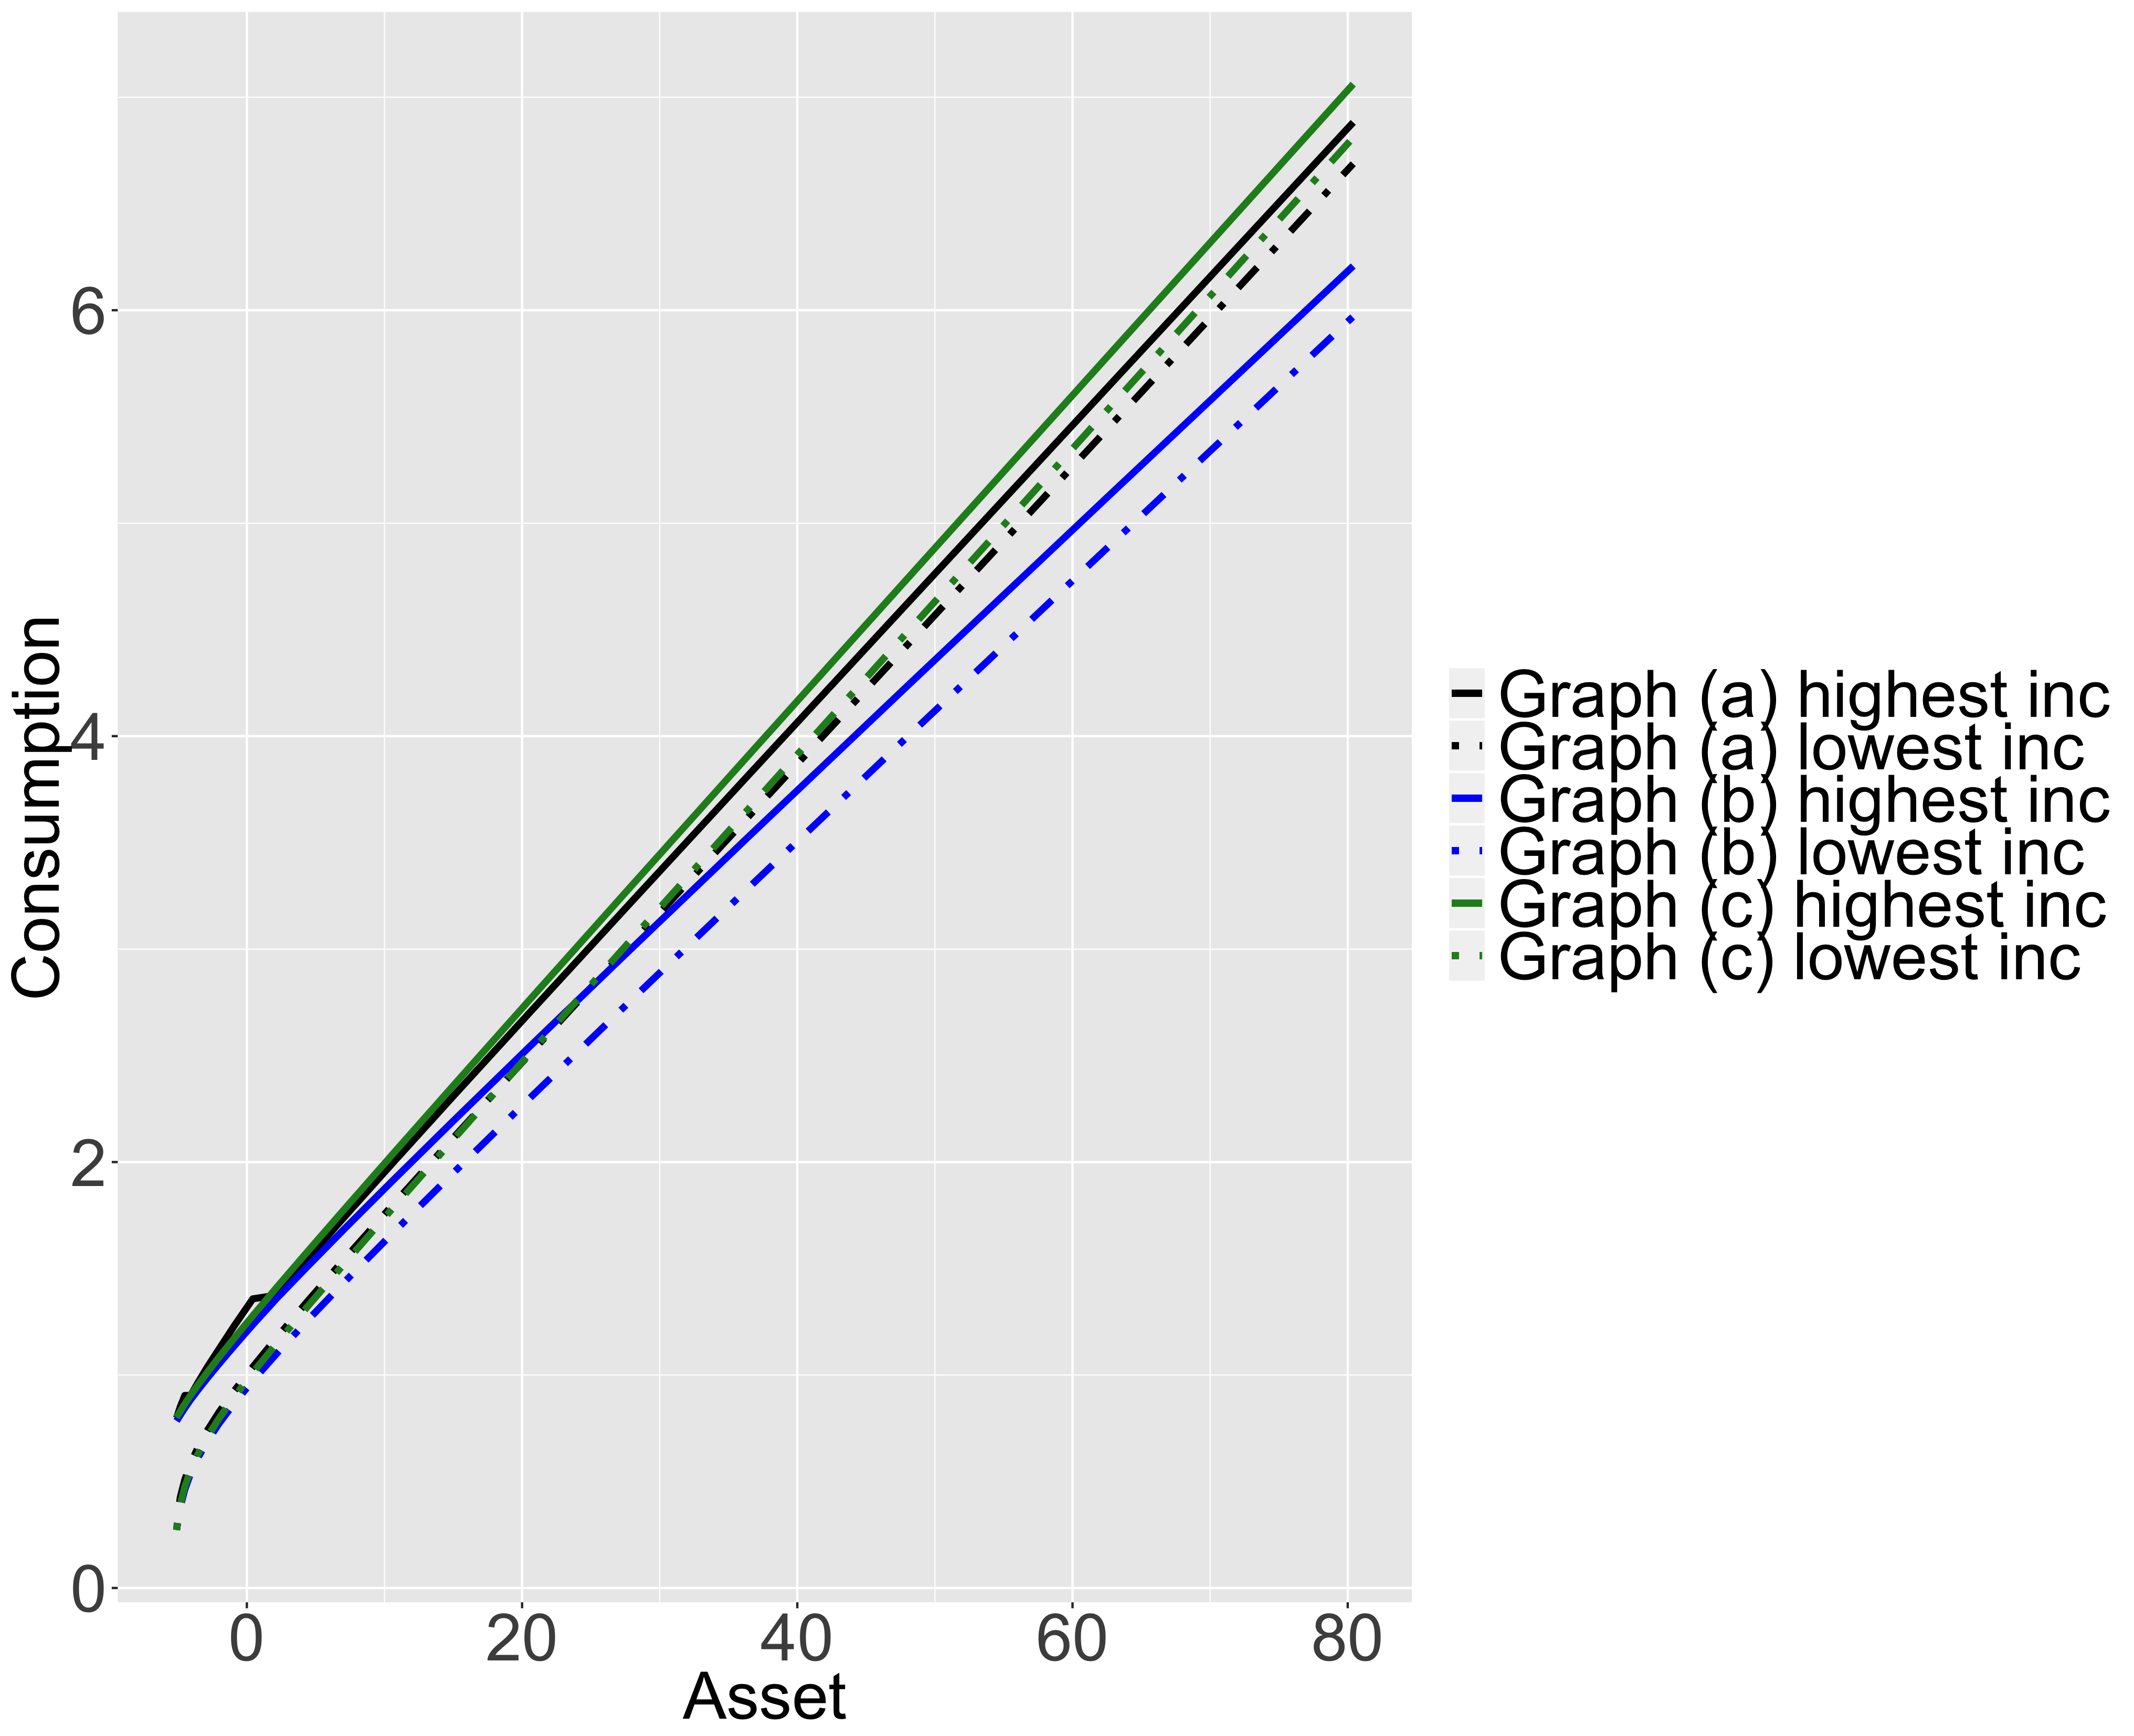
\includegraphics[width=0.8\linewidth]{Question2}
\label{fig:question2}
\end{figure}
Due to numerical errors, graph (a) and (b) are different from the true optimal consumption plan. However, graph (c) is almost identical with true optimal consumption plan. Using linear transformation helps reducing numerical error.\\

\textbf{Question 3. Simulating consumption and asset path using the solution} \\
\begin{figure}[H]
\centering
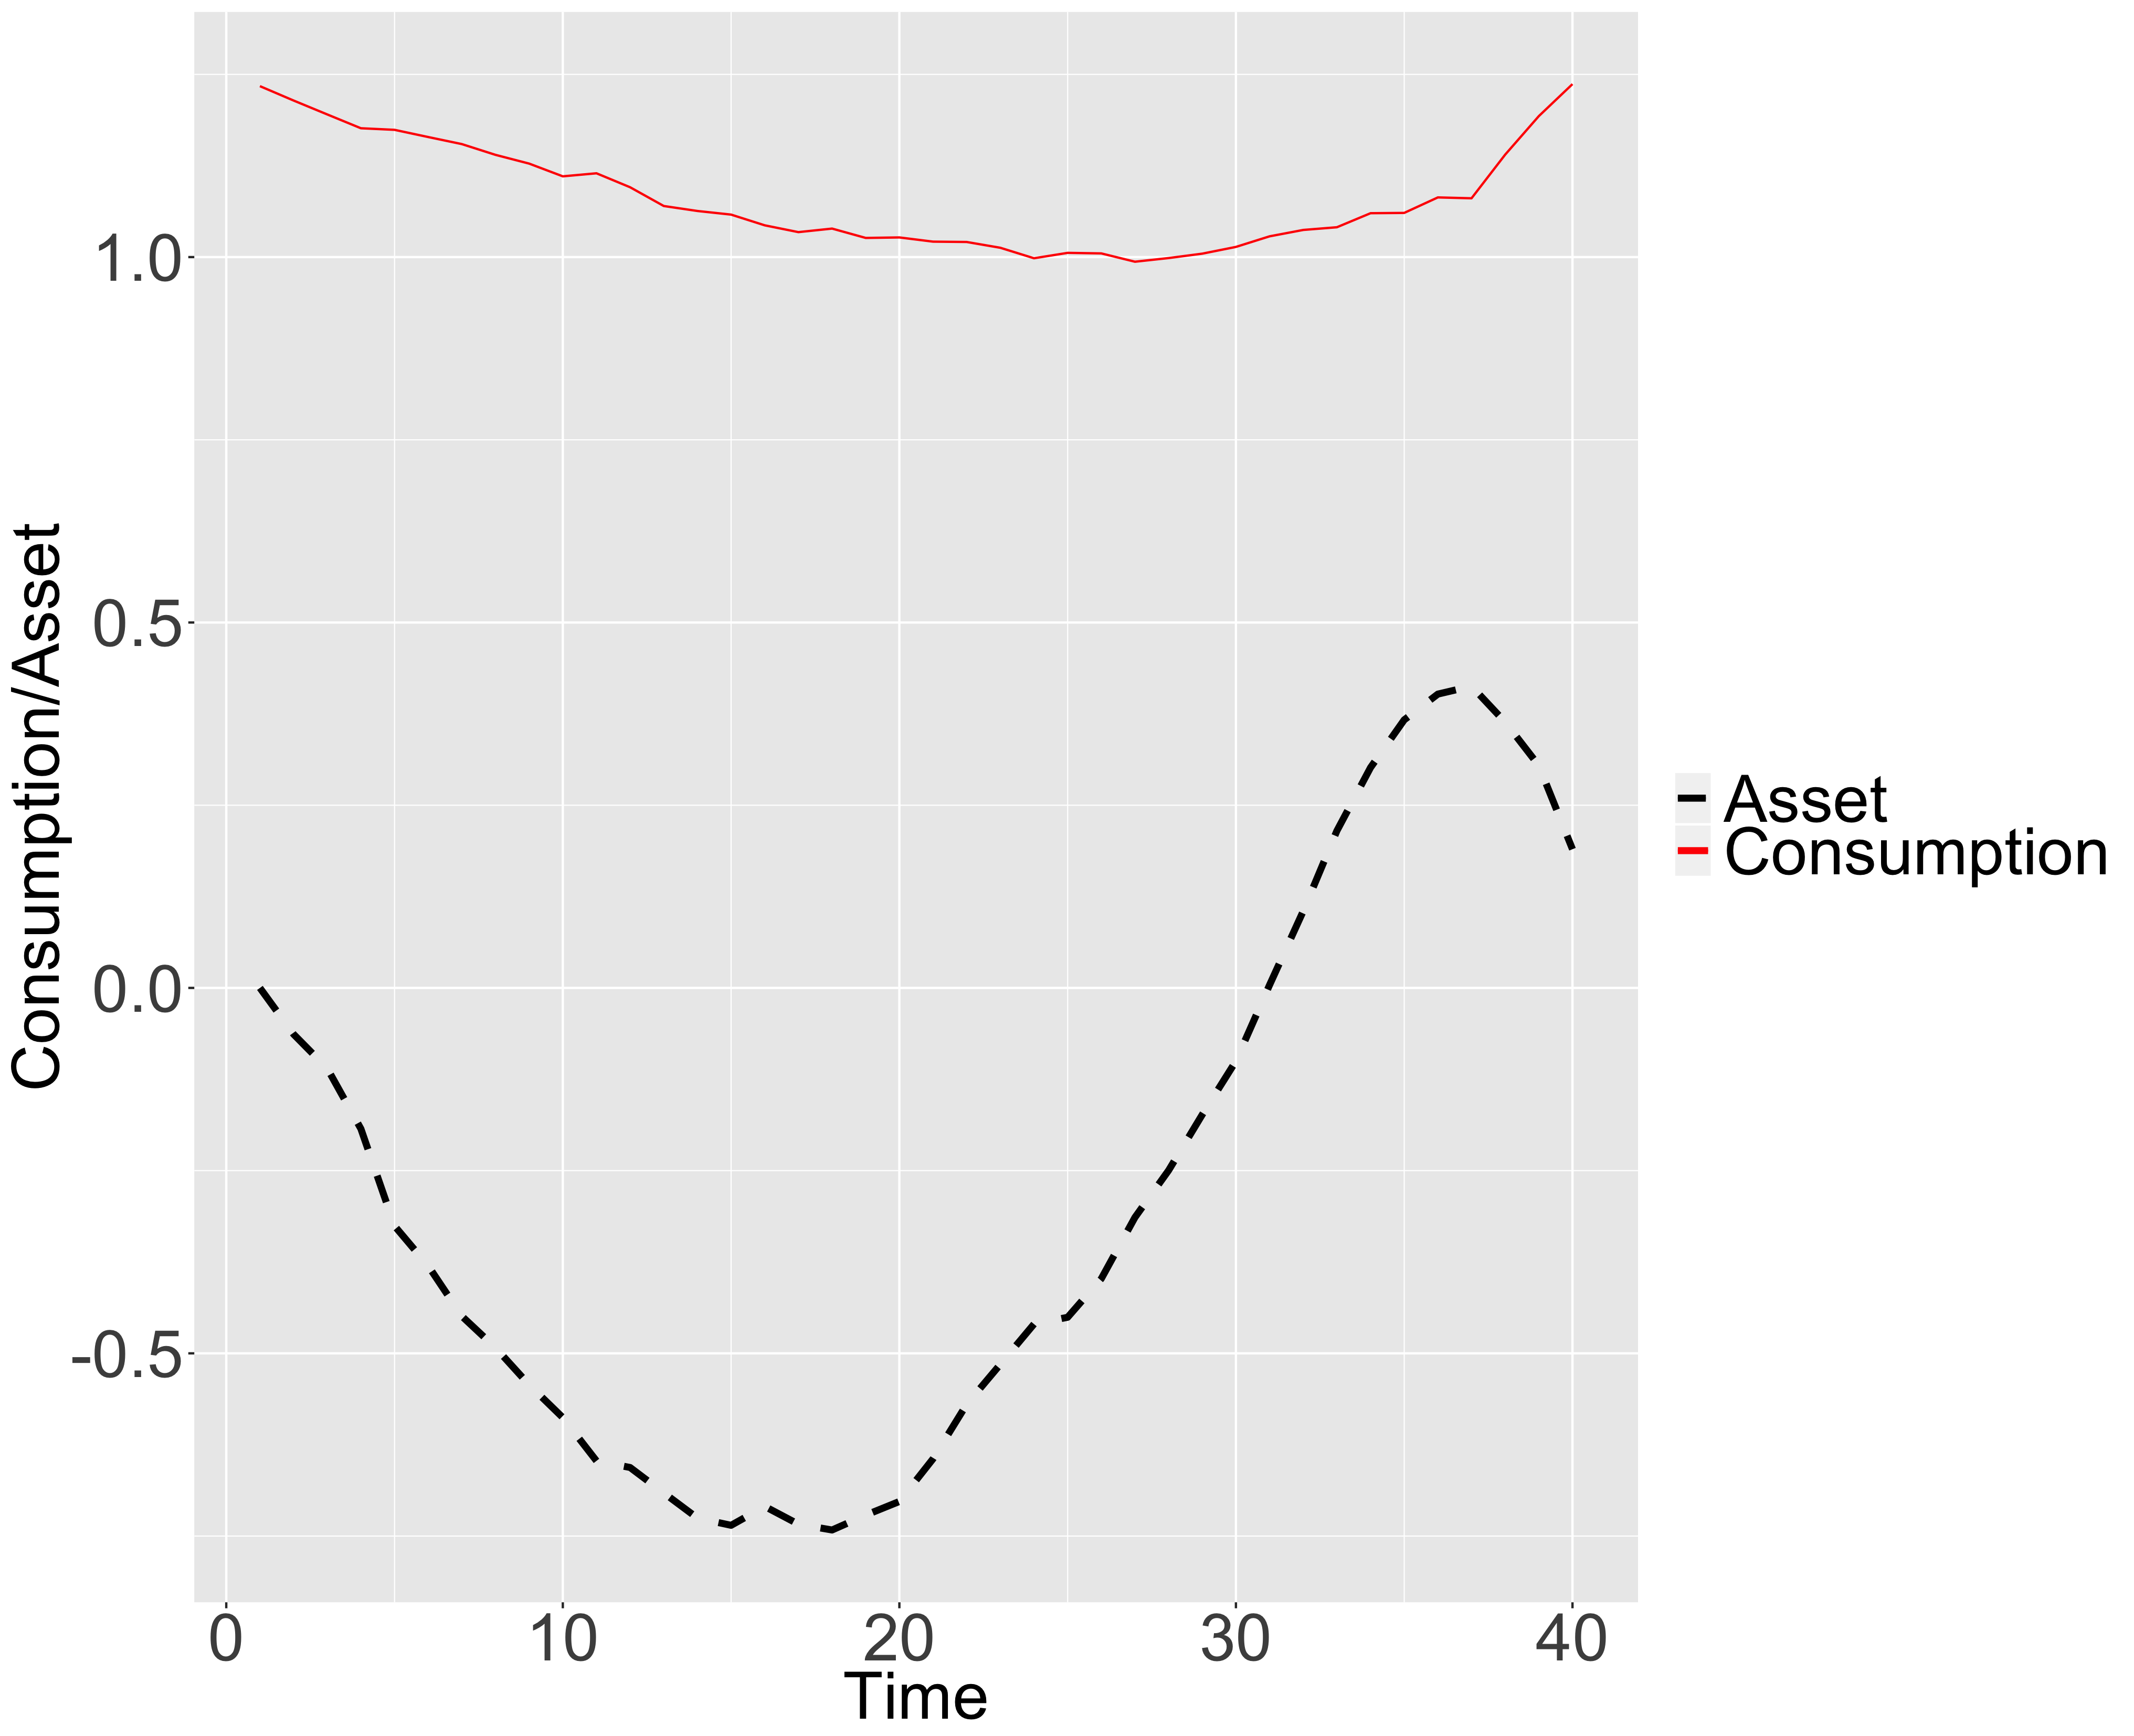
\includegraphics[width=0.8\linewidth]{Question3}
\label{fig:question3}
\end{figure}

\end{document}